\chapter{Approach}


% Describe the performed solution with all possible details. Define necessary parameters, inputs, outputs and context of use, possible problems and when they can be applied. 

% Remember to define necessary concepts before using them, building the text from easiest definitions (not depending on previous definitions) to complex definitions (depending on previous definitions).

% E.g: 
% \begin{itemize}
%	\item Lost Communication: a lost communication occurs when the conditions of the environment are not sufficient or the distance between sender and receiver is to hight to transmit information.
%	\item Wait until rescue: when the robot loses its communication, the pre-designed state machine will stop the motors to keep the actual position. Energy safe mode will be enabled, at the same time that a channel transceiver daemon will send SOS messages every T and wait for reply during T sec. 
%\end{itemize}

The challenge is how to coordinate multiple robots to execute a set of tasks. To tackele this problem, a communication efficient scheduler system is designed, where each robot autonomously request task from the centralized scheduler and centralized scheduler response with a set of suitable tasks. The architecture of this centralized scheduler is shown in \ref{fig:system_architecture}.


\begin{figure}[htb]
	\centering
	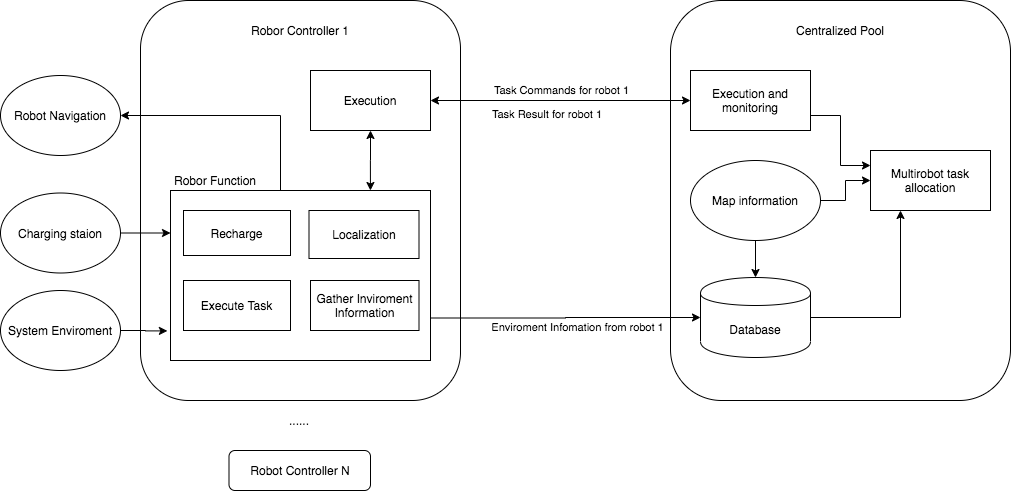
\includegraphics[width = 0.6\textwidth]{content/images/ch3/architecture.drawio.png}
	\caption{System architecture}
	\label{fig:system_architecture}
\end{figure}

\section{The System Components}



\begin{figure}[htb]
	\centering
	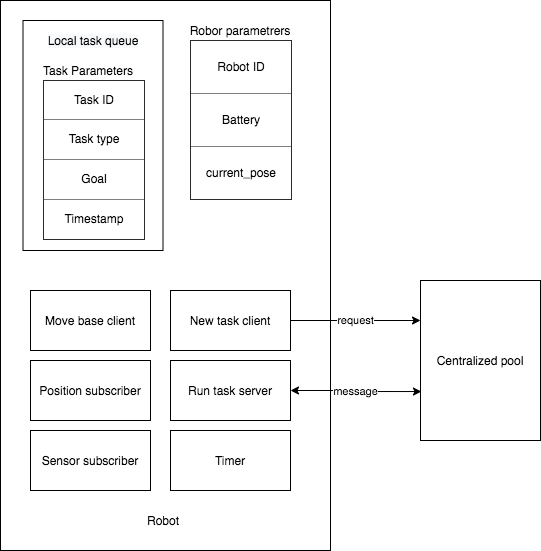
\includegraphics[width = 0.45\textwidth]{content/images/ch3/system_component_robot.drawio.png}
	\caption{Robot Components}
	\label{fig:robot_components}
\end{figure}

\begin{itemize}
	\item \textsl{Robot ID.} Robot ID is a unique identification for each robot.
	\item \textsl{Battery level.} Battery level drops as the robot moves and rotates.
	\item \textsl{Task type.} Robots perform different tasks such as "Charging", "Execute Task", "Gather Enviroment Information". For details please refer to 
	\item \textsl{Local task queue.} Local task queue keeps a list of tasks that a robot will run sequentially. Once the robot finish a task is finished, it would remove the from task queue. Once this queue become empty, the robot send task result to centralized pool.
	\item \textsl{New task client.} After a robot finishing a task, the new task client send new task request to new task server.
	\item \textsl{Run task server.} The run task server receive tasks and send task feedback and task result.
	\item \textsl{Timer.} To prevent robot to be hanged by one task forever, the timer check the robot moving state periodically.
	\item \textsl{Move base client.} The move\_base node provides a ROS interface for configuring, running, and interacting with the navigation stack on a robot. The move\_base client send a goal to move\_base node to tracking their status  
	\item \textsl{Position subscriber} The position subscriber get robot current position from navigation stack. The robot send its current location to centralized pool to request a new task.
	\item \textsl{Sensor subscriber} The Sensor subscriber listen to sensor data within the range.
\end{itemize}

\begin{figure}[htb]
	\centering
	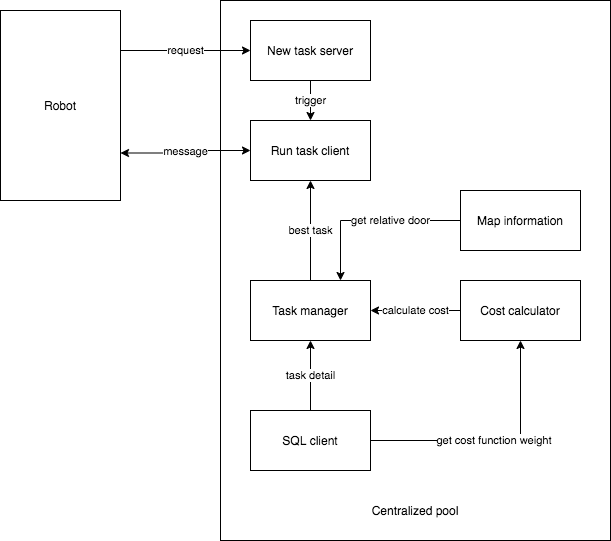
\includegraphics[width = 0.45\textwidth]{content/images/ch3/system_component_centralized_pool.drawio.png}
	\caption{Centralized Pool Components}
	\label{fig:centralized_pool_components}
\end{figure}


